\paperchapter{December 2003}{7 December 2003}{C}{50}{GSET 2003}
\keytable{\kcell{1}{B} & \kcell{2}{B} & \kcell{3}{C} & \kcell{4}{A} & \kcell{5}{D} & \kcell{6}{D} & \kcell{7}{D} & \kcell{8}{B} & \kcell{9}{A} & \kcell{10}{D} \\
\kcell{11}{C} & \kcell{12}{B} & \kcell{13}{A} & \kcell{14}{C} & \kcell{15}{B} & \kcell{16}{A} & \kcell{17}{C} & \kcell{18}{B} & \kcell{19}{A} & \kcell{20}{B} \\
\kcell{21}{C} & \kcell{22}{A} & \kcell{23}{B} & \kcell{24}{B} & \kcell{25}{A} & \kcell{26}{C} & \kcell{27}{D} & \kcell{28}{D} & \kcell{29}{D} & \kcell{30}{B} \\
\kcell{31}{C} & \kcell{32}{D} & \kcell{33}{B} & \kcell{34}{B} & \kcell{35}{C} & \kcell{36}{C} & \kcell{37}{D} & \kcell{38}{D} & \kcell{39}{B} & \kcell{40}{D} \\
\kcell{41}{C} & \kcell{42}{B} & \kcell{43}{D} & \kcell{44}{C} & \kcell{45}{D} & \kcell{46}{D} & \kcell{47}{B} & \kcell{48}{B} & \kcell{49}{C} & \kcell{50}{B}}
\begin{context}
\textbf{Q.~1--5:} The table below shows the number of students admitted to different colleges I, II, III, IV and V in a particular session in various disciplines. Refer to the table to answer the questions 1--5 that follow.
\begin{center}\small
\begin{tabular}{lccccc|c}\toprule \textbf{Discipline} & MBA & B.Tech & B.Sc. & B.Com. & B.A. & \\
\textbf{Capacity} & 200 & 200 & 400 & 300 & 500 & \textbf{1600}\\\midrule
College I & 185 & 200 & 312 & 281 & 486 & 1464\\ College II & 190 & 183 & 348 & 215 & 414 & 1350\\ College III & 198 & 191 & 364 & 291 & 484 & 1528\\ College IV & 170 & 178 & 290 & 199 & 429 & 1266\\ College V & 167 & 199 & 377 & 276 & 412 & 1431\\\bottomrule
\multicolumn{7}{l}{\scriptsize Last column (total admitted) added for the solutions.}
\end{tabular}
\end{center}
\end{context}
\begin{question}{1}
{How many seats in all disciplines taken together are vacant in colleges II and III?\par}
\optsfour{278}{322}{612}{None of these}
\answer{B}{322}
\begin{explain}
Vacant in II $=1600-1350=250$; vacant in III $=1600-1528=72$. Total $=\mathbf{322}$.
\end{explain}
\end{question}

\begin{question}{2}
{What is the approximate difference between the percentage of students admitted to a discipline in respective colleges showing the lowest admission to B.Sc.\ and the highest admission in B.A.?\par}
\optsfour{19\%}{25\%}{34\%}{29\%}
\answer{B}{25\%}
\begin{explain}
Lowest B.Sc.\ admission: College IV, $290/400=72.5\%$. Highest B.A.: College I, $486/500=97.2\%$. Difference $=24.7\%\approx\mathbf{25\%}$.
\end{explain}
\end{question}

\begin{question}{3}
{Which of the following colleges has the highest number of vacant seats in Commerce and Arts discipline ?\par}
\optsfour{II}{III}{IV}{V}
\answer{C}{IV}
\begin{explain}
Vacant seats in B.Com.\ $+$ B.A.: II $=85+86=171$; III $=9+16=25$; \textbf{IV $=101+71=172$}; V $=24+88=112$. The highest is \textbf{IV}.
\end{explain}
\end{question}

\begin{question}{4}
{What is the difference in the percentage of students admitted in M.B.A. of Colleges II and IV?\par}
\optsfour{10\%}{12\%}{15\%}{20\%}
\answer{A}{10\%}
\begin{explain}
MBA: II $=190/200=95\%$; IV $=170/200=85\%$. Difference $=\mathbf{10\%}$.
\end{explain}
\end{question}

\begin{question}{5}
{What is the total percentage of seats vacant in college III against its total capacity?\par}
\optsfour{6.86\%}{5.36\%}{3.92\%}{4.37\%}
\answer{D}{4.37\%}
\keynote{From the table, College III has $72/1600=4.5\%$ seats vacant; the nearest option, and the official key, is (D) 4.37\%.}
\begin{explain}
Vacant seats in College III $=1600-1528=72$; $\dfrac{72}{1600}\times100=4.5\%$. The key gives the nearest option, \textbf{4.37\%}.
\end{explain}
\end{question}

\begin{context}
\textbf{Q.~6--10:} In the following figure, the \textbf{circle} stands for medical students, the \textbf{square} for hardworking, the \textbf{triangle} for rural and the \textbf{rectangle} (tilted) for affluents. Pick out the numeral associated with the region.
\begin{center}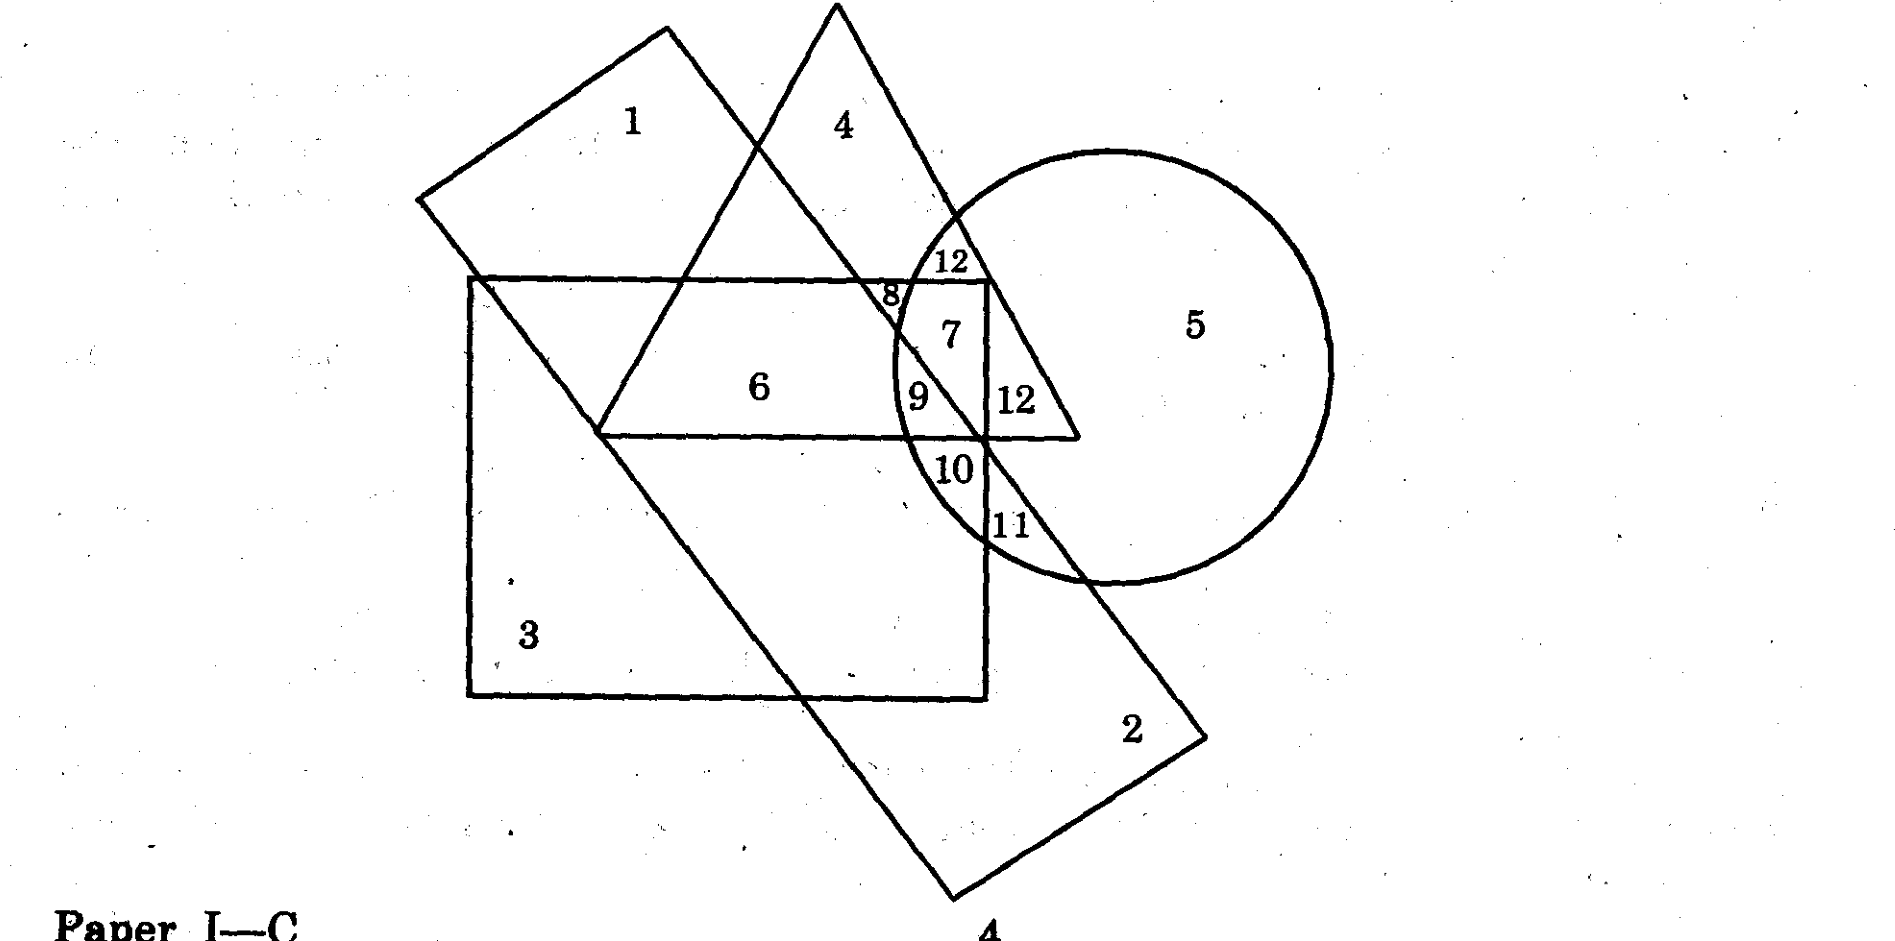
\includegraphics[width=0.72\linewidth]{fig/dec03_q6.png}\end{center}
\end{context}
\begin{question}{6}
{Non-rural and hardworking medical students who are affluent are represented by the region:\par}
\optsfour{5}{7}{9}{10}
\answer{D}{10}
\begin{explain}
Required: inside circle, square and tilted rectangle, but \textbf{outside the triangle}. That is region \textbf{10}.
\tip{Method for every such question: list the figures the region must be \emph{inside} and those it must be \emph{outside}, then find the single numbered region that satisfies all conditions.}
\end{explain}
\end{question}

\begin{question}{7}
{Medical students who are neither affluent nor hardworking but are rural are represented by the region :\par}
\optsfour{8}{10}{11}{12}
\answer{D}{12}
\begin{explain}
Inside circle and triangle; outside square and rectangle: region \textbf{12} (the part of the triangle inside the circle but above/right of the square and rectangle).
\end{explain}
\end{question}

\begin{question}{8}
{Hardworking, non-affluent rural medical students are represented by the region:\par}
\optsfour{6}{7}{9}{12}
\answer{B}{7}
\begin{explain}
Inside circle, square and triangle; outside the rectangle: region \textbf{7}.
\end{explain}
\end{question}

\begin{question}{9}
{Non-affluent medical students who are not hardworking and who do not belong to rural areas are represented by the region :\par}
\optsfour{5}{6}{8}{11}
\answer{A}{5}
\begin{explain}
Inside the circle only (outside square, triangle and rectangle): region \textbf{5}.
\end{explain}
\end{question}

\begin{question}{10}
{Medical students who are affluent, hardworking and rural are represented through the region:\par}
\optsfour{6}{8}{9}{10}
\answer{D}{10}
\begin{explain}
Inside all four figures (circle, square, triangle, rectangle): region \textbf{9}.
\end{explain}
\end{question}

\begin{question}{11}
{Complete the number series given below: 320, 320, 160, 40, ?\par}
\optsfour{4}{0}{5}{10}
\answer{C}{5}
\begin{explain}
Divide successively by 1, 2, 4, 8: $320\div1=320$, $\div2=160$, $\div4=40$, $\div8=\mathbf{5}$.
\end{explain}
\end{question}

\begin{question}{12}
{Complete the number series given below: 1, 5, 45, 445, ?\par}
\optsfour{4545}{4445}{5454}{4455}
\answer{B}{4445}
\begin{explain}
Each term $=$ previous $\times10-5$: $1\rightarrow5\rightarrow45\rightarrow445\rightarrow\mathbf{4445}$.
\end{explain}
\end{question}

\begin{question}{13}
{Which of the following will come next in the series given below: BHL, DJN, FLP, ?\par}
\optsfour{HNR}{HOS}{IOS}{INR}
\answer{A}{HNR}
\begin{explain}
Each letter advances by 2: B$\rightarrow$D$\rightarrow$F$\rightarrow$\textbf{H}, H$\rightarrow$J$\rightarrow$L$\rightarrow$\textbf{N}, L$\rightarrow$N$\rightarrow$P$\rightarrow$\textbf{R}. Next: \textbf{HNR}.
\end{explain}
\end{question}

\begin{question}{14}
{Which of the following will come next in the series given below: KUZ, MOX, OIV, QET, ?\par}
\optsfour{SUR}{SAQ}{RAR}{SAR}
\answer{C}{RAR}
\begin{explain}
First letters K, M, O, Q, \textbf{S} ($+2$); last letters Z, X, V, T, \textbf{R} ($-2$); middle letters U, O, I, E, \textbf{A} (moving back through the vowels). Next: \textbf{SAR}.
\end{explain}
\end{question}

\begin{question}{15}
{In the following letter sequence, find the correct alternative for the missing letters: ab.\ldots{}cba.\ldots{}bcc.\ldots{}aab.\ldots{}cba.\ldots{}b\par}
\optsfour{bbbba}{cabca}{caacb}{babcb}
\answer{B}{cabca}
\begin{explain}
Filling c, a, b, c, a gives
\[\text{ab\underline{c}cba\underline{a}bcc\underline{b}aab\underline{c}cba\underline{a}b}=\text{abccba}\,|\,\text{abccba}\,|\,\text{abccba}\,|\,\text{ab}\]
The block ``abccba'' repeats, so the answer is \textbf{cabca}.
\end{explain}
\end{question}

\begin{question}{16}
{In the following letter sequence, find the correct alternative for the missing letters: ab.\ldots{}abc.\ldots{}cab.\ldots{}bc.\ldots{}b\par}
\optsfour{cabcaa}{baabbc}{caaccc}{cachca}
\answer{A}{cabcaa}
\begin{explain}
Filling the gaps with c, a, b, c, a, a (option A) completes the repeating letter pattern built from ``abc''. Answer as per key: \textbf{cabcaa}.
\end{explain}
\end{question}

\begin{question}{17}
{A cube is painted red on two opposite faces and green on two adjacent faces. The remaining two faces are left uncoloured. It is cut into 125 equal cubes. How many cubes have green colour on one face only?\par}
\optsfour{16}{19}{24}{40}
\answer{C}{24}
\begin{explain}
The cube is cut $5\times5\times5$. Let top and bottom be red, front and right green, left and back uncoloured.
On the front (green) face, remove the top row and bottom row (also red) and the column on the right edge (also green): $3\times4=12$ cubes have green only. Same for the right face.
Total $=12\times2=\mathbf{24}$.
\end{explain}
\end{question}

\begin{question}{18}
{Referring to the cube described in Q17: How many cubes are coloured green on two faces ?\par}
\optsfour{2}{5}{7}{9}
\answer{B}{5}
\begin{explain}
Cubes with green on two faces lie along the common edge of the two green faces: $\mathbf{5}$ cubes (the two end cubes on this edge are also red, but they still carry green on two faces).
\end{explain}
\end{question}

\begin{question}{19}
{In the multiplication given below, find the digits corresponding to the letters:\\[3pt]
\centering\begin{tabular}{r} 6 b c\\ $\times$\ 3 5 d\\\hline 6 6 e\\ 3 3 3 0\ \ \\ 1 a a 8\ \ \ \ \\\hline 2 2 3 7 6 6\end{tabular}\\[3pt]
\raggedright `b' stands for:\par}
\optsfour{6}{7}{8}{9}
\answer{A}{6}
\begin{explain}
The second partial product is $6bc\times5=3330$, so $6bc=666$. Hence \textbf{b $=$ 6} (and c $=6$, d $=1$, e $=6$, a $=9$: $666\times3=1998$).
\end{explain}
\end{question}

\begin{question}{20}
{In the same multiplication, `c' stands for:\par}
\optsfour{7}{6}{5}{4}
\answer{B}{6}
\begin{explain}
From $6bc=666$ (because $6bc\times5=3330$): \textbf{c $=$ 6}.
\end{explain}
\end{question}

\begin{context}
\textbf{Q.~21--22:} A square cardboard ABCD, inside which the square JKLM is inscribed, is placed horizontally (and may be reversed). In each question, two conditions are given: (I) whether the cardboard is reversed; (II) the direction of one vertex with respect to the centre O. Find the direction of the other given vertex with respect to O.
\begin{center}
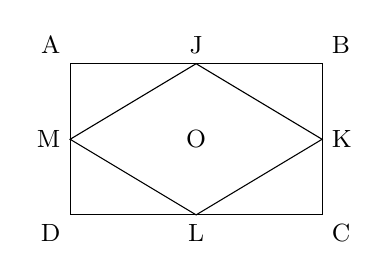
\begin{tikzpicture}[scale=0.8,font=\small]
\draw (0,0) rectangle (4,2.4); \draw (2,2.4)--(4,1.2)--(2,0)--(0,1.2)--cycle;
\node[above left] at (0,2.4){A}; \node[above right] at (4,2.4){B}; \node[below right] at (4,0){C}; \node[below left] at (0,0){D};
\node[above] at (2,2.4){J}; \node[right] at (4,1.2){K}; \node[below] at (2,0){L}; \node[left] at (0,1.2){M}; \node at (2,1.2){O};
\end{tikzpicture}
\end{center}
In the normal position: A $=$ NW, B $=$ NE, C $=$ SE, D $=$ SW; J $=$ N, K $=$ E, L $=$ S, M $=$ W.
\end{context}
\begin{question}{21}
{(I) Not reversed. (II) A towards S. `J' will be in the direction:\par}
\optsfour{N}{W}{SW}{NW}
\answer{C}{SW}
\begin{explain}
A moves from NW to S: a rotation of $225^\circ$ clockwise (NW $\rightarrow$ N $\rightarrow$ \ldots\ $\rightarrow$ S is 5 steps of $45^\circ$). J (N) rotated $225^\circ$ clockwise points \textbf{SW}.
\end{explain}
\end{question}

\begin{question}{22}
{(I) Not reversed. (II) L towards NE. `M' will be in the direction:\par}
\optsfour{SE}{E}{N}{S}
\answer{A}{SE}
\begin{explain}
L moves from S to NE: $225^\circ$ clockwise. M (W) rotated $225^\circ$ clockwise $\rightarrow$ \textbf{SE}.
\end{explain}
\end{question}

\begin{question}{23}
{Six persons I, II, III, IV, V and VI are sitting in a room. Three are females and three are males. I is father of III, III is son of II, III is brother of IV, IV is not son of I, V is nephew of I, VI is niece of II. Who is the daughter of I?\par}
\optsfour{IV}{VI}{III}{None of these}
\answer{B}{VI}
\keynote{By the given relations the daughter of I is IV. The official key gives (B) VI.}
\begin{explain}
I is father of III and II is mother (III is son of II). III is brother of IV, and IV is \emph{not} son of I, so IV is I's \textbf{daughter}. V and VI are nephew and niece (children of a sibling). Logically the answer is IV; the key gives \textbf{VI}.
\end{explain}
\end{question}

\begin{question}{24}
{If GOLD is coded as EMJB, then NMPR will be decoded as\par}
\optsfour{RIOT}{PORT}{ROTS}{PORK}
\answer{B}{PORT}
\begin{explain}
GOLD $\rightarrow$ EMJB: each letter moves 2 back. To decode NMPR, move each letter 2 forward: \textbf{PORT}.
\end{explain}
\end{question}

\begin{question}{25}
{If 6743 is coded as FGDC, then 97285 will be coded as:\par}
\optsfour{IGBHE}{RTYSV}{GVSTU}{IHCIF}
\answer{A}{IGBHE}
\begin{explain}
The code replaces digit $n$ by the $n$-th letter: 6$\rightarrow$F, 7$\rightarrow$G, 4$\rightarrow$D, 3$\rightarrow$C. So 97285 $\rightarrow$ I G B H E $=$ \textbf{IGBHE}.
\end{explain}
\end{question}

\begin{question}{26}
{At a certain restaurant, above the kitchen door four small lights, numbered 1 to 4 from left to right, are used to signal waiters: I $=$ all four lights; II $=$ lights 1 and 2; III $=$ light 1 only; IV $=$ lights 2, 3 and 4; V $=$ lights 3 and 4. Not-working lights are taken as illuminated.\\ If lights two and three both are off, then the waiter signalled could be:\par}
\optsfour{I}{II}{III}{IV}
\answer{C}{III}
\begin{explain}
With lights 2 and 3 off, only signals that do not use 2 or 3 remain: III (light 1 only). \textbf{III}.
\end{explain}
\end{question}

\begin{question}{27}
{If lights one and two are not working (and hence count as illuminated), and lights three and four are illuminated, then the signal of which of the waiters (I, IV and V) might be signalled?\par}
\optsfour{I only}{V only}{I and IV}{I, IV and V}
\answer{D}{I, IV and V}
\begin{explain}
Lights 3 and 4 are on and lights 1 and 2 may or may not be intended, so the signal could be I (all four), IV (2, 3, 4) or V (3, 4): \textbf{I, IV and V}.
\end{explain}
\end{question}

\begin{question}{28}
{Select from the following groups, the word that does not belong to the group:\par}
\optsfour{Tin}{Steel}{Iron}{Copper}
\answer{D}{Copper}
\keynote{Strictly, steel (an alloy) is the odd one out among the metallic elements tin, iron and copper. The official key gives (D) Copper.}
\begin{explain}
Tin, iron and copper are elements; steel is an alloy of iron. The official key, however, gives \textbf{Copper} (the only non-greyish, reddish metal of the group). Mark (D) as per the key.
\end{explain}
\end{question}

\begin{question}{29}
{Find the odd one out of the following:\par}
\optsfour{Truthful}{Sly}{Virtuous}{Pensive}
\answer{D}{Pensive}
\begin{explain}
Truthful, sly and virtuous describe a person's \emph{moral character}. \textbf{Pensive} (thoughtful) describes a \emph{mood}, so it is the odd one.
\end{explain}
\end{question}

\begin{question}{30}
{A watch costs Rs. 800. At what price should a shopkeeper mark up, if after allowing a discount of 10 per cent on the marked up price, he makes a profit of 12.5\% on the cost price ?\par}
\optsfour{Rs. 950}{Rs. 1,000}{Rs. 1,250}{Rs. 1,500}
\answer{B}{Rs. 1,000}
\begin{explain}
Required SP $=800\times1.125=900$. SP $=0.9\times$ MP, so MP $=900/0.9=$ \textbf{Rs.~1,000}.
\end{explain}
\end{question}

\begin{question}{31}
{In a college level instruction, the purpose of selective admission is to:\par}
\optsone{debar those who may create problem to the lecturer}{ensure equality and justice}{screen those who can benefit from higher education}{increase the revenue of the college through admission tests}
\answer{C}{screen those who can benefit from higher education}
\begin{explain}
Selective admission aims to \textbf{screen those who can benefit from higher education}, i.e.\ admit students with the required aptitude and preparation.
\end{explain}
\end{question}

\begin{question}{32}
{A lecturer is planning his/her lecture for a course. Which of the following may be considered least helpful?\par}
\optsone{deciding the content to be delivered}{identifying suitable methodology of presentation}{getting information about his/her students' background}{discussing with his/her principal as to what he/she considers to be the functions of a lecturer}
\answer{D}{discussing with his/her principal as to what he/she considers to be the functions of a lecturer}
\begin{explain}
Per the key, the least helpful step is option (D), discussing the plan with others. Deciding content, choosing methodology and knowing the students' background are essential parts of lecture planning.
\end{explain}
\end{question}

\begin{question}{33}
{During classroom teaching interactive sessions should be encouraged because :\par}
\optsone{teacher's job becomes less challenging during such sessions}{students' involvement is enhanced}{teaching is not everybody's cup of tea}{students should be given some breathing time to learn}
\answer{B}{students' involvement is enhanced}
\begin{explain}
Interactive sessions \textbf{enhance students' involvement}, which improves understanding and retention.
\end{explain}
\end{question}

\begin{question}{34}
{A college or a university should submit itself for evaluation to the National Assessment and Accreditation Council (NAAC) because :\par}
\optsone{It is the need of the hour}{It will enable it to know its strength and weaknesses}{It will justify its existence}{It will help in deciding grants for the college/university}
\answer{B}{It will enable it to know its strength and weaknesses}
\begin{explain}
NAAC evaluation helps an institution \textbf{know its strengths and weaknesses}, so that it can improve quality.
\end{explain}
\end{question}

\begin{question}{35}
{Which of the following pairs of incentives are likely to strongly motivate the adolescents ?\par}
\optstwo{Teacher and parents' approval}{Certificates and academic honours}{Peer and compeer approval}{Principal and teachers' encouragement}
\answer{C}{Peer and compeer approval}
\begin{explain}
Adolescents are strongly influenced by their peer group, so \textbf{peer and compeer approval} is the most powerful incentive.
\end{explain}
\end{question}

\begin{question}{36}
{The office of a Chief Proctor in a university has justification because :\par}
\optsone{There are a number of proctors in a university}{The university ordinance requires it to be so}{Students' activities/programmes need regulatory control}{Students are generally unruly and need control}
\answer{C}{Students' activities/programmes need regulatory control}
\begin{explain}
A Chief Proctor's office is justified because \textbf{students' activities and programmes need regulatory control} (discipline and order on campus).
\end{explain}
\end{question}

\begin{question}{37}
{Which research focusses on improvement of work situations ?\par}
\optstwo{Fundamental Research}{Applied Research}{Survey Research}{Action Research}
\answer{D}{Action Research}
\begin{explain}
\textbf{Action research} focuses on improving one's own work situation or practice.
\end{explain}
\end{question}

\begin{question}{38}
{The need for sampling in research arises because :\par}
\optstwo{It is economical}{It is time-saving}{It improves accuracy of results}{All the above considerations hold}
\answer{D}{All the above considerations hold}
\begin{explain}
Sampling is economical, saves time, and (because a smaller group can be studied more carefully) can improve accuracy: \textbf{all the above}.
\end{explain}
\end{question}

\begin{question}{39}
{A researcher has collected data in form of cross breaks by setting up a 2 x 3 table in terms of frequency counts. Which of the following tests will be most appropriate for arriving at an appropriate analysis ?\par}
\optsone{Parametric tests}{Non-parametric tests}{Both parametric and non-parametric tests}{Logical tests}
\answer{B}{Non-parametric tests}
\begin{explain}
Frequency counts in a $2\times3$ contingency table call for the \textbf{chi-square test}, a non-parametric test.
\end{explain}
\end{question}

\begin{question}{40}
{In reporting research findings the main purpose should be to:\par}
\optstwo{meet the sponsorer's expectations}{help other researchers}{attract public attention}{highlight the factual position}
\answer{D}{highlight the factual position}
\begin{explain}
The main purpose of reporting research is to \textbf{highlight the factual position}, i.e.\ to present the findings honestly and objectively.
\end{explain}
\end{question}

\begin{question}{41}
{Select the word that is the nearest equivalent to the capitalized word: ABDICATE :\par}
\optsfour{Plead}{Censure}{Renounce}{Abolish}
\answer{C}{Renounce}
\begin{explain}
\textbf{Abdicate} means to give up (a throne or responsibility), i.e.\ \textbf{renounce}.
\end{explain}
\end{question}

\begin{question}{42}
{Select the word that is the nearest equivalent to the capitalized word: SHAM:\par}
\optsfour{Lovable}{Pretence}{Guilty}{Jittery}
\answer{B}{Pretence}
\begin{explain}
\textbf{Sham} means something false or fake, i.e.\ \textbf{pretence}.
\end{explain}
\end{question}

\begin{question}{43}
{In arriving at knowledge through the method of research, which of the following combinations is most appropriate ?\par}
\optstwo{Authority + Inductive reasoning}{Experience + Deductive reasoning}{Creativity + Deductive reasoning}{Inductive + Deductive reasoning}
\answer{D}{Inductive + Deductive reasoning}
\begin{explain}
The research method combines \textbf{inductive and deductive reasoning} (the reflective or scientific method).
\end{explain}
\end{question}

\begin{question}{44}
{Select the lettered pair wherein the words have the closest relationship to that of the numbered pair: Information : Feedback ::\par}
\optstwo{Gun : Recoil}{Letter : Reply}{Action : Reaction}{Aborigines : Boomerang}
\answer{C}{Action : Reaction}
\begin{explain}
Feedback is the response that comes back to information. Similarly, reaction is the response to \textbf{action}.
\end{explain}
\end{question}

\begin{question}{45}
{Select the lettered pair wherein the words have the closest relationship to that of the numbered pair: Activate : Detonate ::\par}
\optstwo{Inform : Deform}{Engage : Disengage}{Quicken : Mutilate}{Deaden : Diffuse}
\answer{D}{Deaden : Diffuse}
\begin{explain}
Per the official key, the pair is \textbf{Deaden : Diffuse}, i.e.\ the second word is the (intensified) result of the first, as detonation follows activation.
\end{explain}
\end{question}

\begin{context}
\textbf{Q.~46--50:} Read the passage given below and answer the questions.\par\smallskip
Competition the world over is slowly becoming a lethal agent in killing the regenerative process among human beings. This is happening through a vicious cycle of anxiety--tension--stress--depression--nervous breakdown. The problem percolates to the entire human structure touching health of the body, mind and spirit. To prepare a sound mind in a sound body is a coveted definition of education. But in the present life-cycle dynamics everything seems to explode. More so for those aspiring to be competitive winners irrespective of the field, the killer instinct is soon becoming a self killing process. Much has been spoken and written about the evil effects of stress and its psychosomatic repercussions. Many solutions have been offered by counselling agencies across the globe --- some bordering on spiritual remedies, while large chunk depending upon psychiatric-psychic process. Many have also recommended physical activity to control stress and depression. However, an integrated approach to life management programme in the competitive environment could probably be the most easy and efficient course of remedy. But what is not clearly taken into reckoning is the fact that the body, the mind and the spirit all the three together form an individual and therefore, the health of each of these three components is equally important and has a separate existence. For instance, when the mind is disturbed, thereby creating unhealthiness in the intellectual-emotional plane, the body despite being in absolute physical comfort still gets affected and is often the victim. Therefore, it is necessary to understand fear and conquer it at the first place in order to arrest spread of anxiety, stress, tension and depression.
\end{context}
\begin{question}{46}
{Basic objective of this passage is to project:\par}
\optstwo{Ways of remaining healthy}{Avoidance of anxiety}{Avoidance of competitive spirit}{Causes of mental ill health}
\answer{D}{Causes of mental ill health}
\begin{explain}
The passage traces how competition produces anxiety, stress and depression and affects body, mind and spirit, i.e.\ the \textbf{causes of mental ill health}.
\end{explain}
\end{question}

\begin{question}{47}
{After going through this passage, two premises come up. You are to indicate which is right.\\
I. Anxiety leads to nervous breakdown.\\ II. Stress has evil effects on health.\par}
\optstwo{I is right and II is wrong}{I is wrong and II is right}{I and II both are right}{I and II both are wrong}
\answer{B}{I is wrong and II is right}
\begin{explain}
Per the key, only II is right: the passage directly states the ``evil effects of stress and its psychosomatic repercussions''. Anxiety is only the first link of a cycle, not directly said to cause breakdown.
\end{explain}
\end{question}

\begin{question}{48}
{The whole passage is structured in the form which may be called:\par}
\optsfour{Narrative}{Explanatory}{Analytical}{Expository}
\answer{B}{Explanatory}
\begin{explain}
The passage explains a problem, its causes and possible remedies, so it is \textbf{explanatory}.
\end{explain}
\end{question}

\begin{question}{49}
{The most appropriate title for the passage would be :\par}
\optstwo{Evil effects of competition}{Managing good health}{Overcoming stress}{Managing good living}
\answer{C}{Overcoming stress}
\begin{explain}
The passage ends with the need to understand fear and arrest stress, anxiety and depression, so the best title is \textbf{Overcoming Stress}.
\end{explain}
\end{question}

\begin{question}{50}
{In the passage the words 'Disturbed Mind' can be suitably replaced by the words:\par}
\optsfour{Activated Mind}{Agitated Mind}{Unhealthy Mind}{Anxious Mind}
\answer{B}{Agitated Mind}
\begin{explain}
A ``disturbed mind'' is an \textbf{agitated mind}.
\end{explain}
\end{question}
